\section{Einzelne Tabellen abfragen mit \texorpdfstring{\gls{SQL}}{SQL}}

\lstset{style=sql}

\subsection{Syntax}
Die Sprache \acrfull{SQL} besteht, wie wir sehen werden, aus verschiedenen Schlüsselwörtern, wie etwa \lstinline|SELECT|, \lstinline|WHERE|, \lstinline|GROUP BY|, \lstinline|ORDER BY| usw. Dazu gibt es Folgendes zu beachten:
\begin{itemize}
  \item Ob wir diese Schlüsselwörter gross oder klein schreiben, spielt keine Rolle. Allerdings wird empfohlen, die Schlüsselwörter immer in Grossbuchstaben zu schreiben, um sie von Kolonnen-Namen, Tabellen-Namen usw. abzugrenzen.
  \item Wir können alle \gls{SQL}-Befehle auf einer einzigen Zeile schreiben, dadurch wird der Code aber deutlich weniger lesbar. Stattdessen empfiehlt es sich, vor gewissen Schlüsselwörtern wie \lstinline|SELECT|, \lstinline|WHERE| oder \lstinline|GROUP BY| eine neue Zeile zu erstellen. Dazu lohnt es sich, die Beispiele genau anzuschauen.
\end{itemize}

\textbf{Kommentare} können in \gls{SQL}  auf zwei Arten geschrieben werden:

\begin{lstlisting}
-- 1. Kommentar auf einer Zeile
/* 2. Kommentar über
mehrere Zeilen */
\end{lstlisting}

% need to add "texorpdfstring" to avoid warnings
\subsection{Einfache Selektion: \texorpdfstring{\lstinline|SELECT|}{SELECT}}

Mit dem Befehl \enquote{\lstinline|SELECT col1,col2,... FROM tablename|} können wir gewisse Spalten ($=$ Kolonnen) \lstinline|col1,col2,...| aus einer Tabelle mit dem Namen \lstinline|tablename| auswählen. Wir können statt den Spaltennamen auch einfach einen Stern (\texttt{*}) tippen, um alle Kolonnen einer Tabelle zu erhalten, d.h. die gesamte Tabelle.


\begin{myexample}
Geben Sie auf InstaHub den folgenden Befehl ein (der \textcolor{blue}{Kommentar} muss nicht kopiert werden, er dient lediglich zur Erklärung des Codes):

\begin{lstlisting}
-- wähle alle Spalten aus der Tabelle users aus
SELECT *
FROM users
\end{lstlisting}

Mit diesem Befehl wählen wir alle Spalten (\lstinline|*|) der Tabelle \lstinline|users| aus.
Sie sollten nun die gesamte Tabelle \texttt{users} sehen.
\end{myexample}

\begin{myexercise}
  Geben Sie alle Benutzernamen (\texttt{username}) aus \texttt{users} aus.
  \begin{myanswer}
    \begin{lstlisting}
      SELECT username
      FROM users
      \end{lstlisting}
  \end{myanswer}
\end{myexercise}

\begin{myexercise}
  Geben Sie die Benutzernamen (\texttt{username}) und echten Namen (\texttt{name}) aller Einträge aus \texttt{users} aus.
  \begin{myanswer}
    \begin{lstlisting}
      SELECT username, name
      FROM users
    \end{lstlisting}
  \end{myanswer}
\end{myexercise}

\begin{myexercise}
  Geben Sie die Namen und Wohnorte aller Mitglieder aus.
  \begin{myanswer}
    \begin{lstlisting}
      SELECT username, city
      FROM users
    \end{lstlisting}
  \end{myanswer}
\end{myexercise}

\subsection{Selektion mit Filter: \texorpdfstring{\lstinline|WHERE|}{WHERE}}
Fügen wir zu einer \gls{SQL}-Abfrage den Befehl ``\lstinline|WHERE conditions|'' hinzu, können wir das erhaltene Resultat nach gewissen Bedingungen (\texttt{conditions}) filtern.

\begin{myexample}
Geben Sie folgendes Beispiel in Instahub ein:

\begin{lstlisting}
SELECT name, city, gender
FROM users
WHERE gender="male"
\end{lstlisting}
\end{myexample}

Nebst dem Gleich-Zeichen (im obigen Beispiel) stehen folgende Filter-Operatoren zur Verfügung:
\begin{table}[H]
  \centering
  \begin{tabular}{c|l}
    \makecell{\textbf{Operator}                                                                 \\\textbf{in \gls{SQL}}} & \makecell{\textbf{Mathematische}\\\textbf{Bedeutung}} \\\midrule
    \texttt{=}                                    & gleich ($=$)                                \\
    \texttt{<>}                                   & ungleich ($\neq$)                           \\
    \texttt{<}                                    & kleiner als ($<$)                           \\
    \texttt{<=}                                   & kleiner oder gleich ($\leq$)                \\
    \texttt{>}                                    & grösser als ($>$)                           \\
    \texttt{>=}                                   & grösser oder gleich ($\geq$)                \\
    \lstinline|BETWEEN x AND y|        & ein Wert zwischen (inklusive) \texttt{x} und \texttt{y} \\
    \lstinline|IN (wert1, wert2, ...)| & einer von mehreren möglichen Werten         \\
    \lstinline|IS NULL|                & Wert existiert nicht                        \\
  \end{tabular}
\end{table}
Um mehrere Bedingungen miteinander zu verknüpfen, können wir die Befehle \lstinline|AND|, \lstinline|NOT| sowie \lstinline|OR| verwenden.
%TODO: braucht es eine Erklärung zu Klammern für die richtige Verknüpfung von mehreren Bedingungen?

\begin{myexample}\label{myexample:between}
Folgender Code gibt alle Mitglieder aus, die zwischen 172 cm und 174 cm gross sind. Dabei gehören 172 cm und 174 cm selbst ebenfalls dazu (inklusive).

\begin{lstlisting}
SELECT name, centimeters, gender 
FROM users 
WHERE centimeters BETWEEN 172 AND 174 
\end{lstlisting}
\end{myexample}

\begin{myexample}\label{myexample:in}
Folgender Code gibt den Namen und die Stadt aller Mitglieder aus, die entweder in Leipzig, Berlin oder Hamburg wohnen.

\begin{lstlisting}
SELECT name, city
FROM users 
WHERE city IN ("Leipzig", "Berlin", "Hamburg")
\end{lstlisting}
\end{myexample}


\begin{mycaution}
Wie Sie anhand der \cref{myexample:in,myexample:between} sehen, spielt es in SQL eine Rolle, ob  wir nach Zahlen oder nach
  Text filtern: Wenn nach einem Text gefiltert wird, muss dieser in Anführungszeichen stehen (wie z.B.
  \lstinline|"Berlin"| in \cref{myexample:in}). Bei Zahlen dürfen Sie keine Anführungszeichen schreiben (s. z.B. die Zahl
  \lstinline|172| in \cref{myexample:between}).
\end{mycaution}

\lstinline|NULL| ist ein spezielles \gls{SQL}-Wort, welches bedeutet, dass ein Feld leer ist, bzw. keinen
Wert hat. \lstinline|NULL| muss von \enquote{0} unterschieden werden: Beispielsweise könnte die Zahl 0 in einer 
Tabelle über Bankkonten bedeuten, dass jemand 0 Franken auf seinem Konto hat, während der Wert \lstinline|NULL| bedeuten würde, dass keine 
Informationen zum Kontostand vorhanden sind.

\begin{myexample}
  Folgender Code gibt die Namen aller Mitglieder an, die ihre Grösse nicht angegeben haben.
\begin{lstlisting}
SELECT name, centimeters
FROM users 
WHERE centimeters IS NULL
\end{lstlisting}
\end{myexample}


\begin{myexercise}
  Geben Sie die Namen aller weiblichen Mitglieder aus, die zwischen 150 und 155 gross sind.
  \begin{myanswer}
    \begin{lstlisting}
      SELECT name, gender, centimeters
      FROM users
      WHERE gender="female"
      AND centimeters BETWEEN 150 AND 155
    \end{lstlisting}
  \end{myanswer}
\end{myexercise}
\begin{myexercise}
  Zeigen Sie den Namen, das Geburtsdatum sowie die Grössen aller Frauen an, die kleiner oder gleich 160 Zentimeter sind.
  \begin{myanswer}
    \begin{lstlisting}
      SELECT name, birthday, centimeters
      FROM users
      WHERE gender="female"
      AND centimeters <= 160
    \end{lstlisting}
  \end{myanswer}
\end{myexercise}

\begin{myexercise}
  Verwenden Sie die Tabelle \texttt{comments} und geben Sie alle Kommentare aus, die vom user mit der ID 10 oder vom user mit der ID 38 stammen.
  \begin{myanswer}
    \begin{lstlisting}
      SELECT user_id, body 
      FROM comments 
      WHERE user_id IN (38, 10)
\end{lstlisting}
  \end{myanswer}
\end{myexercise}


\subsection{Eindeutige Selektion: \texorpdfstring{\lstinline|SELECT DISTINCT|}{SELECT DISTINCT}}

Der Befehl \lstinline|DISTINCT| nach einem \lstinline|SELECT| führt dazu, dass jeder mögliche Wert
nur höchstens einmal ausgegeben wird, d.h. Duplikate werden entfernt.

\begin{myexercise}
  Vergleichen Sie folgende zwei Befehle. Überlegen Sie sich zuerst, was der Code ausgeben sollte, bevor Sie die Befehle in InstaHub ausführen.

 \begin{lstlisting}
SELECT gender
FROM users
\end{lstlisting}

  \begin{lstlisting}
SELECT DISTINCT gender
FROM users
\end{lstlisting}
\end{myexercise}

\begin{myexercise}
  Geben Sie jeden Wohnort nur einmal aus.
  \begin{myanswer}
    \begin{lstlisting}
SELECT DISTINCT city 
FROM users
\end{lstlisting}
  \end{myanswer}
\end{myexercise}
\begin{myexercise}
  Geben Sie jede Benutzerrolle nur einmal aus. \texttt{dba} bedeutet ``Database Administrator'', also Datenbank-AdministratorIn.
  \begin{myanswer}
    \begin{lstlisting}
SELECT DISTINCT role
FROM users
\end{lstlisting}
  \end{myanswer}
\end{myexercise}


\subsection{Ungefähre Treffer: \texorpdfstring{\lstinline|LIKE|}{LIKE}}

Mit dem Befehl \lstinline|LIKE| können wir die Tabelle nach Zeilen filtern, welche in einer gewissen Spalte ein bestimmtes Wort enthalten.

\begin{myexample}
Mit folgendem Befehl erhalten wir alle Städte, die mit ``Be'' beginnen:

\begin{lstlisting}
SELECT DISTINCT city 
FROM users 
WHERE city LIKE "Be%"
\end{lstlisting}
\end{myexample}

Das ``\%''-Zeichen ist eine sogenannte \textit{wildcard} und dient hier als Platzhalter, der Folgendes bedeutet: ``es \textit{kann} noch weiterer Text an dieser Stelle stehen, \textit{muss} aber nicht'' (s. \cref{table:wildcards}).

\begin{table}[ht]
  \centering
  \begin{tabular}{c|l}
    \textbf{Symbol}            & \textbf{Bedeutung}                              \\ \midrule
    \lstinline|"%"| & Stellt null oder mehrere, beliebige Zeichen dar \\ \hline
    \lstinline|"_"| & Stellt ein einzelnes, beliebiges Zeichen dar    \\
  \end{tabular}
  \caption{\textit{wildcards} in \gls{SQL}}
  \label{table:wildcards}
\end{table}

\begin{myexample}
Mit folgendem Befehl erhalten wir alle Städte, die mit ``H'' beginnen und ein ``m'' an dritter Stelle haben:

\begin{lstlisting}
SELECT DISTINCT city 
FROM users 
WHERE city LIKE "H_m%"
\end{lstlisting}
\end{myexample}



\begin{myexercise}
  Vergleichen Sie folgende drei Befehle. Überlegen Sie sich zuerst, was der Code ausgeben sollte, bevor sie die Befehle in InstaHub ausführen.

  \begin{lstlisting}
SELECT username, city 
FROM users 
WHERE city = "Berlin" AND name LIKE "Fabian%"
\end{lstlisting}

  \begin{lstlisting}
SELECT username, city 
FROM users 
WHERE city = "Berlin" OR name LIKE "Fabian%"
\end{lstlisting}

  \begin{lstlisting}
SELECT username, city 
FROM users 
WHERE city = "Berlin" AND NOT name LIKE "Fabian%"
\end{lstlisting}
\end{myexercise}

\begin{myexercise}
  Finden Sie alle Berliner, die \textit{Marc} heissen.
  \begin{myanswer}
    \begin{lstlisting}
SELECT name, city
FROM users
WHERE city="Berlin" AND name LIKE "Marc%"
\end{lstlisting}
  \end{myanswer}
\end{myexercise}

\begin{myexercise}
  Finden Sie alle Person mit dem Vornamen \textit{Lina} oder \textit{Lorena}.
  \begin{myanswer}
    \begin{lstlisting}
      SELECT name, city
      FROM users
      WHERE name LIKE "Lina%"
      OR name LIKE "Lorena%"
    \end{lstlisting}
  \end{myanswer}
\end{myexercise}

\begin{mychallenge}
  Überprüfen Sie, welche Mitglieder im Jahr 2001 geboren sind (mit der Spalte \texttt{birthday}).
  \begin{myanswer}
    \begin{lstlisting}
SELECT name, birthday
FROM users
WHERE birthday LIKE "2001%"
\end{lstlisting}
  \end{myanswer}
\end{mychallenge}

% TODO: soll das eine Abgabe sein?
\begin{myexercise}
  Wählen Sie alle Personen mit dem Namen \textit{Naomi} aus, die nicht aus Berlin kommen.
  \begin{myanswer}
    \begin{lstlisting}
SELECT name, city
FROM users
WHERE name LIKE "Naomi%"
AND city <> "Berlin"
\end{lstlisting}
  \end{myanswer}
\end{myexercise}

\begin{mychallenge}
  Geben Sie die Grösse und den Wohnort von Juliette Amsel sowie Juliette Unger aus. Sie sollten das Zeichen \lstinline|"%"| nicht verwenden.
  \begin{myanswer}
    \begin{lstlisting}
SELECT name, centimeters, city
FROM users
WHERE name LIKE "Juliette ___e_"
\end{lstlisting}
  \end{myanswer}
\end{mychallenge}

\subsection{Sortieren: \texorpdfstring{\lstinline|ORDER BY|}{ORDER BY}}

Mit dem Befehl \lstinline|ORDER BY col ASC| oder \lstinline|ORDER BY col DESC| kann das Resultat einer \gls{SQL} -Abfrage nach einer bestimmten Kolonne \lstinline|col| sortiert werden. Mit \lstinline|ASC| wird das Resultat aufsteigend und mit \lstinline|DESC| absteigend sortiert.

\begin{myexample}
Beobachten Sie das Resultat folgender Abfrage:

\begin{lstlisting}
SELECT DISTINCT city 
FROM users 
ORDER BY city DESC
\end{lstlisting}
\end{myexample}

\begin{myexercise}
  Geben Sie alle Benutzernamen in sortierter Reihenfolge aus (a $\rightarrow$ z).
  \begin{myanswer}
    \begin{lstlisting}
SELECT username
FROM users
ORDER BY username ASC
\end{lstlisting}
  \end{myanswer}
\end{myexercise}

\begin{mysubmission}
  \begin{itemize}
    \item Lösen Sie Aufgaben 1--11 unter folgendem Link:\\
\url{https://sql-tutorial.de/home/uebungen.php?lektion=1} (keine Abgabe notwendig / möglich)
    \item Geben Sie danach auf Moodle die ``Übungen 1 (Einfache Selektion)'' ab.
  \end{itemize}
\end{mysubmission}

\subsection{Aggregatsfunktionen}

\subsubsection{\texorpdfstring{\lstinline|COUNT|}{COUNT}}

Mit dem Befehl \lstinline|COUNT| kann man die Anzahl Resultate zählen.

\begin{lstlisting}
SELECT COUNT(*)
FROM users
\end{lstlisting}

Wir können den berechneten Wert zudem zur besseren Lesbarkeit umbenennen, indem wir den Befehl \lstinline|AS| verwenden:

\begin{lstlisting}
SELECT COUNT(*) AS "Registrierte Mitglieder" 
FROM users
\end{lstlisting}

\begin{myexercise}
  Geben Sie die Anzahl registrierten Mitglieder in Berlin aus. Die resultierende Spalte soll ``Registrierte Mitglieder in Berlin'' heissen.
  \begin{myanswer}
    \begin{lstlisting}
SELECT COUNT(*) AS "Registrierte Mitglieder in Berlin" 
FROM users
WHERE city="Berlin"
\end{lstlisting}
  \end{myanswer}
\end{myexercise}

\subsubsection{\texorpdfstring{\lstinline|MAX, MIN|}{MAX, MIN}}

Um die höchsten, bzw. tiefsten Werte einer Kolonne zu erhalten, können die Befehle \lstinline|MIN| und \lstinline|MAX| verwendet werden:

\begin{myexample}
Beobachten Sie das Resultat folgender Abfrage:

\begin{lstlisting}
SELECT MAX(centimeters) AS "Maximale Körpergrösse" 
FROM users
\end{lstlisting}
\end{myexample}

\begin{myexercise}
  Zeigen Sie, wie gross das kleinste Mitglied ist.
  \begin{myanswer}
    \begin{lstlisting}
SELECT MIN(centimeters) AS "Kleinste Körpergrösse"
FROM users
\end{lstlisting}
  \end{myanswer}
\end{myexercise}
\begin{myexercise}
  Zeigen Sie, wann sich zuletzt ein Mitglied registriert hat.
  \begin{myanswer}
    \begin{lstlisting}
SELECT max(created_at) AS "Zuletzt Registriert"
FROM users
\end{lstlisting}
  \end{myanswer}
\end{myexercise}


\subsubsection{\texorpdfstring{\lstinline|SUM|}{SUM}}

Mit \lstinline|SUM| kann die Summe einer Datenserie ausgegeben werden.

\begin{myexample}
Folgender Code berechnet die Summe der Körpergrössen aller Personen, die Felix heissen:

\begin{lstlisting}
SELECT SUM(centimeters) 
FROM users 
WHERE name LIKE "Felix%"
\end{lstlisting}
\end{myexample}

\subsubsection{\texorpdfstring{\lstinline|AVG|}{AVG}}

Mit \lstinline|AVG| kann der Durchschnitt einer Datenserie ausgegeben werden.

\begin{myexample}
Folgender Code berechnet die durchschnittliche Körpergrössen aller Personen, die Felix heissen:

\begin{lstlisting}
SELECT AVG(centimeters) 
FROM users 
WHERE name LIKE "Felix%"
\end{lstlisting}
\end{myexample}

\subsubsection{\texorpdfstring{\lstinline|LENGTH|}{LENGTH}}

Mit \lstinline|LENGTH| gibt die Anzahl Zeichen eines Texts zurück.

\begin{myexample}
Folgender Code berechnet die Länge aller Namen:

\begin{lstlisting}
SELECT name, LENGTH(name) 
FROM users
\end{lstlisting}
\end{myexample}

\begin{mysubmission}
  \begin{itemize}
    \item Lösen Sie Aufgaben 1--6 unter folgendem Link: \url{https://sql-tutorial.de/home/uebungen.php?lektion=2} (keine Abgabe notwendig / möglich)
    \item Geben Sie danach auf Moodle die ``Übungen 2 (Aggregatsfunktionen)'' ab.
  \end{itemize}
\end{mysubmission}

\subsection{Gruppieren: \texorpdfstring{\lstinline|GROUP BY|}{GROUP BY}}
Um die Resultate einer Anfrage pro Untergruppen zu sehen, kann der Befehl \lstinline|GROUP BY| verwendet werden.

\begin{myexample}
Folgender Code gibt die Anzahl Mitglieder pro Stadt aus:
\begin{lstlisting}
SELECT city, COUNT(*) AS "Mitglieder pro Stadt" 
FROM users 
GROUP BY city
\end{lstlisting}
\end{myexample}

Zudem ist es möglich, Daten auch in Untergruppen zusammenzufassen.

\begin{myexample}
Folgender Code gibt die Anzahl männlicher und weiblicher Mitglieder pro Stadt aus:
\begin{lstlisting}
SELECT city, gender, COUNT(*) 
FROM users 
GROUP by city, gender
\end{lstlisting}
\end{myexample}

\subsection{Filtern nach Gruppieren: \texorpdfstring{\lstinline|HAVING|}{HAVING}}
Falls nach einem \lstinline|GROUP BY| die Resultate noch weiter eingegrenzt werden sollen, muss statt \lstinline|WHERE| der Befehl \lstinline|HAVING| verwendet werden. Der Befehl \lstinline|WHERE| wird verwendet, um die ursprünglichen Daten \textit{vor} einem \lstinline|GROUP BY| zu filtern, der Befehl \lstinline|HAVING| wird verwendet, um die Resultate \textit{nach} einem \lstinline|GROUP BY| zu filtern.

\begin{mychallenge}
  Geben Sie die durchschnittliche Körpergrösse aller Mitglieder in jeder Stadt aus. Zeigen Sie nur die Städte, in denen die Menschen im Durchschnitt zwischen 150 und 155 gross sind.
  \begin{myanswer}
    \begin{lstlisting}
SELECT city, AVG(centimeters) AS "Durchschnittliche Körpergrösse"
FROM users
GROUP BY city
HAVING `Durchschnittliche Körpergrösse` BETWEEN 150 AND 155
\end{lstlisting}
  \end{myanswer}
\end{mychallenge}

\begin{mychallenge}
  Geben Sie die maximale Körpergrösse aus, gruppiert nach Stadt und Geschlecht, für alle Städte, die mit dem Buchstaben "B" beginnen
  \begin{myanswer}
    \begin{lstlisting}
SELECT city, gender, MAX(centimeters) AS "Grösste Körpergrösse"
FROM users
WHERE city LIKE "B%"
GROUP BY city, gender
\end{lstlisting}
  \end{myanswer}
\end{mychallenge}

\subsection{Erste / Letzte Zeilen: \texorpdfstring{\lstinline|LIMIT|}{LIMIT}}
Mit dem Befehl \lstinline|LIMIT n| kann das Resultat einer beliebigen \gls{SQL}-Abfrage auf eine gewisse Anzahl Zeilen beschränkt werden. Dies bedeutet, dass das Resultat nach den ersten \texttt{n} Zeilen abgeschnitten wird. Der Befehl steht immer am Ende einer SQL-Abfrage.

Beobachten Sie das Resultat folgender Abfrage:

\begin{myexercise}
  Zeigen Sie nur 3 Mitglieder (nur deren Namen) an.
  \begin{myanswer}
    \begin{lstlisting}
SELECT name
FROM users
LIMIT 3
\end{lstlisting}
  \end{myanswer}
\end{myexercise}

\begin{myexercise}
  Geben Sie die drei Städte mit den meisten Mitgliedern an.
  \begin{myanswer}
    \begin{lstlisting}
SELECT city, COUNT(*) AS "Anzahl Mitglieder"
FROM users
GROUP BY city
ORDER BY `Anzahl Mitglieder` DESC
LIMIT 3
\end{lstlisting}
  \end{myanswer}
\end{myexercise}

\begin{myexercise}
  Zeigen Sie die Namen und Körpergrösse der 5 grössten Mitglieder an.
  \begin{myanswer}
    \begin{lstlisting}
SELECT name, centimeters
FROM users
ORDER BY centimeters DESC
LIMIT 5
\end{lstlisting}
  \end{myanswer}
\end{myexercise}

\begin{mychallenge}
  Geben Sie die Stadtnamen aus, wo die meisten Mitglieder mit einem ``b'' im Namen wohnen (nur die ersten drei Zeilen).

  \textbf{Tipps:}
  \begin{itemize}
    \item Berechnen Sie zuerst mit einem \lstinline|GROUP BY|-Befehl die Anzahl Einwohner pro Stadt
    \item Beschränken Sie danach Ihre Abfrage mit dem \lstinline|WHERE|-Befehl auf Benutzer, die ein ``b'' im Namen haben
    \item Sortieren Sie dann nach der Anzahl Mitglieder
    \item Verwenden Sie den \lstinline|LIMIT|-Befehl erst am Schluss
  \end{itemize}

  \begin{myanswer}
    \begin{lstlisting}
SELECT city, COUNT(*) AS "Mitglieder"
FROM users 
WHERE name LIKE "%b%" 
GROUP by city 
ORDER BY Mitglieder DESC
LIMIT 3
\end{lstlisting}
  \end{myanswer}
\end{mychallenge}

\begin{mysubmission}
  \begin{itemize}
    \item Lösen Sie Aufgaben 1--5 unter folgendem Link: \url{https://sql-tutorial.de/home/uebungen.php?lektion=4}.   
    \item Geben Sie danach auf Moodle ``Übungen 3 (\lstinline|GROUP BY|)'' ab.
  \end{itemize}
\end{mysubmission}

\subsection{Verzweigungen: \texorpdfstring{\lstinline|CASE WHEN|}{CASE WHEN}}

Der SQL-Befehl \lstinline|CASE WHEN| kann helfen, Ausdrücke basierend auf Bedingungen zu schreiben, also ähnlich wie if-elif-else-Verzweigungen in Python.

\begin{myexample}
Die durchschnittliche Körpergrösse in Deutschland beträgt 179 cm für Männer. Folgender Code berechnet für alle Männer, ob sie grösser, kleiner oder gleich dem Durchschnitt sind, und gibt das Resultat in einer neuen Kolonne aus.

\begin{lstlisting}
SELECT name, centimeters,
CASE 
	WHEN centimeters > 179 THEN 'Gross'
    WHEN centimeters < 179 THEN 'Klein'
    ELSE 'Genau im Durchschnitt'
END AS Durchschnittlich
FROM users
WHERE gender="male"
\end{lstlisting}
\end{myexample}

\begin{myexercise}
  Berechnen Sie eine neue Kolonne, die den Text ``langer Name'' enthält, falls ein Name länger als 20 Zeichen lang ist, und ansonsten ``kurzer Name''. BenutzerInnen mit langem Namen sollen zuoberst stehen. Zeigen Sie nur die ersten 5 Zeilen.
  \begin{myanswer}
    \begin{lstlisting}
SELECT name, LENGTH(name),
CASE
	WHEN LENGTH(name)>20 THEN "Langer Name"
    ELSE "Kurzer Name"
END AS "Langer oder kurzer Name"
FROM users
ORDER BY `Langer oder kurzer Name` DESC
LIMIT 5
\end{lstlisting}
  \end{myanswer}
\end{myexercise}

\subsection{Anwendung: Personalisierte Werbung auf InstaHub}

Auf InstaHub können Werbungen an verschiedene User angepasst werden. Dafür sind auf InstaHub noch einige weitere Tabellen angelegt, deren \gls{ERM} in \cref{fig:erm-ads} abgebildet ist.

\begin{figure}[H]
  \centering
  \begin{tikzpicture}[auto]
    % Style for the entities
    \tikzstyle{entity} = [rectangle, draw, thick, minimum width=1cm, minimum height=0.5cm]

    % Style for the relationships
    \tikzstyle{relationship} = [diamond, draw, thick, aspect=2, minimum width=1.5cm, minimum height=0.5cm]

    % Nodes
    \node[entity] (ads) at (0,0) {ads};
    \node[entity] (users) at (4,0) {users};
    \node[entity] (photos) at (10,0) {photos};
    \node[relationship] (analytics) at (7,0) {analytics};

    % Edges
    \draw (users) -- (analytics) node[midway, above] {n};
    \draw (analytics) -- (photos) node[midway, above] {m};

    % There are no visible connections to the 'ads' entity in the provided diagram.
    % If 'ads' is supposed to be connected to 'users' or another entity, the code should be modified accordingly.

  \end{tikzpicture}
  \caption{\gls{ERM} für den Werbe-Teil von InstaHub}
  \label{fig:erm-ads}
\end{figure}

Mit der Tabelle \texttt{analytics} beginnt InstaHub das Verhalten der Besucher zu überwachen. Dabei wird der Besuch von Photo-Detailansichten mit folgenden Werten dokumentiert:

\begin{table}[H]
  \centering
  \begin{tabular}{r|l}
    \textbf{Feld}                 & \textbf{Beschreibung}                                                 \\\midrule
    \commandbox|id|               & Primärschlüssel, fortlaufende Nummer                                  \\
    \hline
    \commandbox|ip|               & Die ersten drei Blöcke der IPv4-Adresse                               \\
    \hline
    \commandbox|device|           & desktop, mobile, tablet oder bot                                      \\
    \hline
    \commandbox|brand_family|     & wird oft nur bei Smartphones mitgesendet, etwa Apple oder Samsung     \\
    \hline
    \commandbox|brand_model|      & wird oft nur bei Smartphones mitgesendet, etwa GALAXY S5              \\
    \hline
    \commandbox|browser_family|   & Broswer (Firefox, Chrome, Safari...)                                       \\
    \hline
    \commandbox|browser_version|  & Versionsnummer des Browsers                                       \\
    \hline
    \commandbox|platform_family|  & Betriebssystem (Windows, Mac, GNU/Linux, iOS, Android...) \\
    \hline
    \commandbox|platform_version| & Die Versionsnummer der Plattform                                      \\
    \hline
    \commandbox|user_id|          & Benutzer, der sich das Foto angesehen hat                              \\
    \hline
    \commandbox|photo_id|         & Angesehenes Foto                                                      \\
    \hline
    \commandbox|created_at|       & Zeitpunkt, als das Foto sich angesehen wurde                          \\
    \hline
    \commandbox|updated_at|       & i.d.R. wie \commandbox|created_at|, nur anders, wenn manuell geändert \\
  \end{tabular}
  \caption{Kolonnen der Tabelle \texttt{analytics}}
\end{table}

Mit diesen Informationen, sowie weiteren Informationen (Hashtags, Geschlecht, Wohnort etc.) kann InstaHub gezielt personalisierte Werbung schalten. Nach diesem Prinzip funktionieren auch andere soziale Medien wie TikTok, Instagram oder Snapchat.

\begin{mycaution}
Für die nachfolgenden Teile müssen Sie, sofern Sie Adblockers in Ihrem Browser verwenden, diese deaktivieren (oder zumindest eine Ausnahme für InstaHub erstellen), da Ihnen die Werbungen ansonsten nicht angezeigt werden.
\end{mycaution}

\clearpage
Auf InstaHub können Werbeanzeigen mit \gls{SQL} personalisiert werden. Dafür geht man zunächst auf die Werbungs-Seite (s. \cref{fig:screenshot-ads1})
\begin{figure}[H]
  \centering
  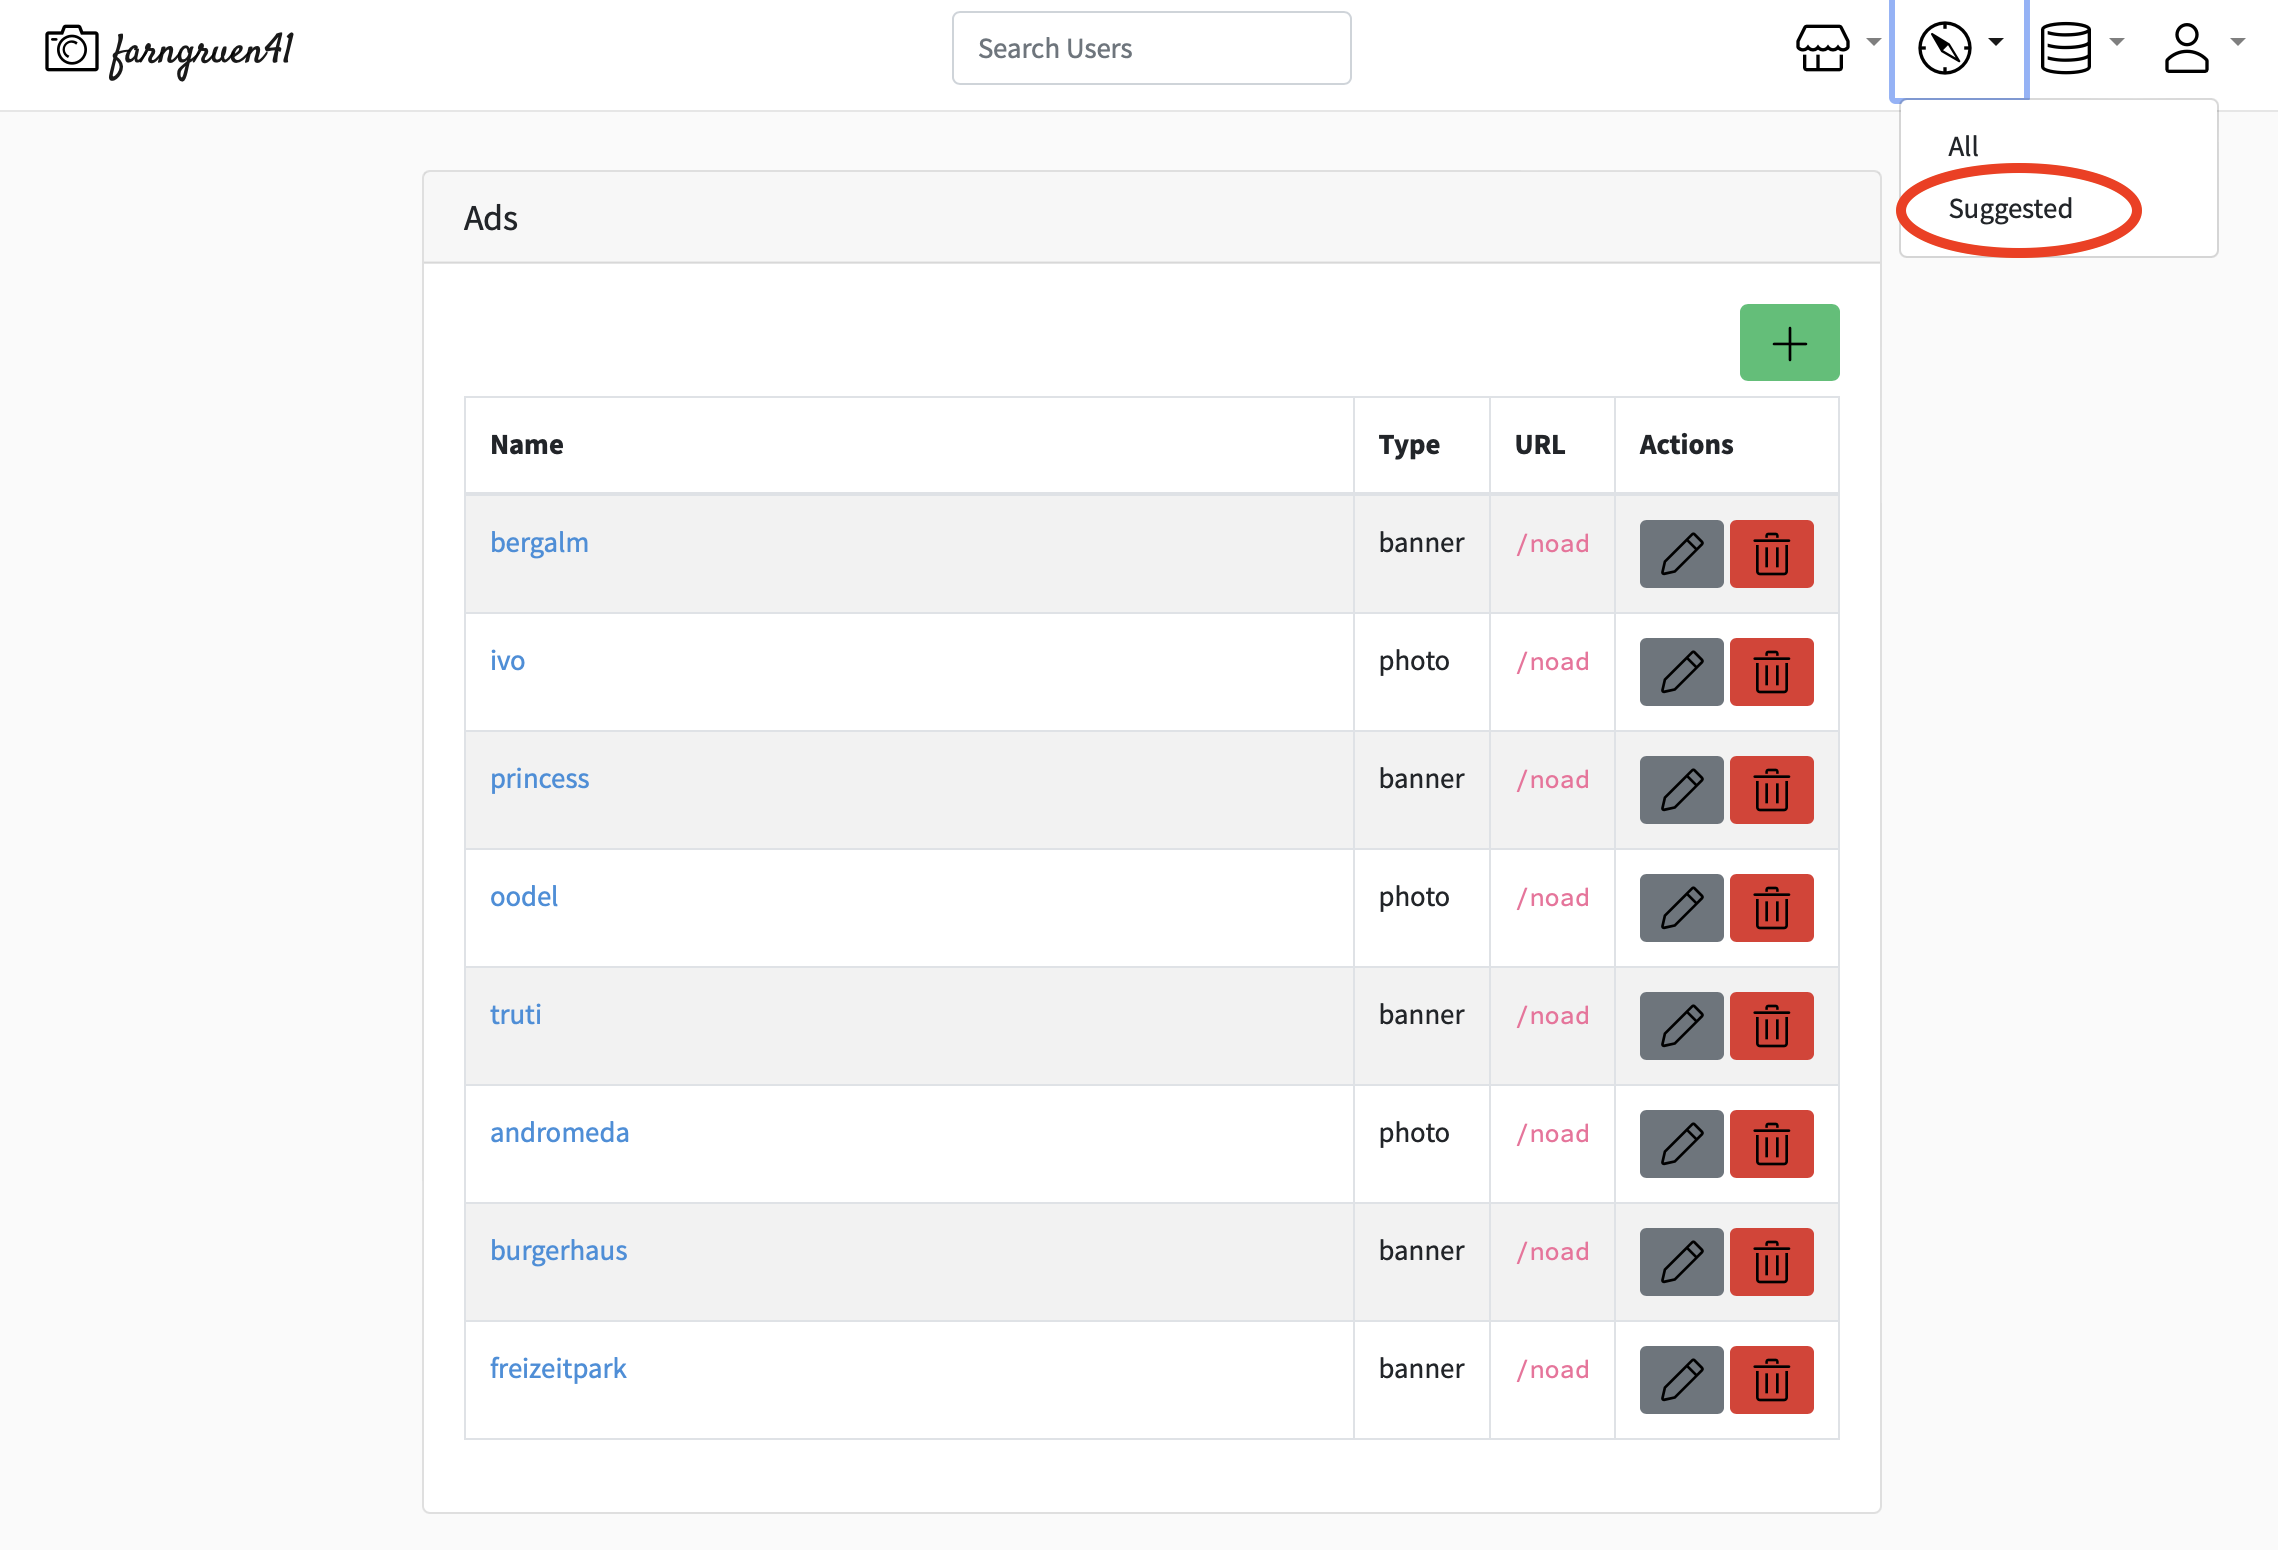
\includegraphics[width=0.7\linewidth]{GrundlagenInfo/06_Daten/Figures/screenshot-ads1}
  \caption{Übersicht der existierenden Werbungs-Kampagnen}
  \label{fig:screenshot-ads1}
\end{figure}

Von dort aus kann man auf eine Werbekampagne klicken, um mehr Details zu sehen. Die Detail-Ansicht der ersten Kampagne ist abgebildet auf \cref{fig:screenshot-ads2}.

\begin{figure}[H]
  \centering
  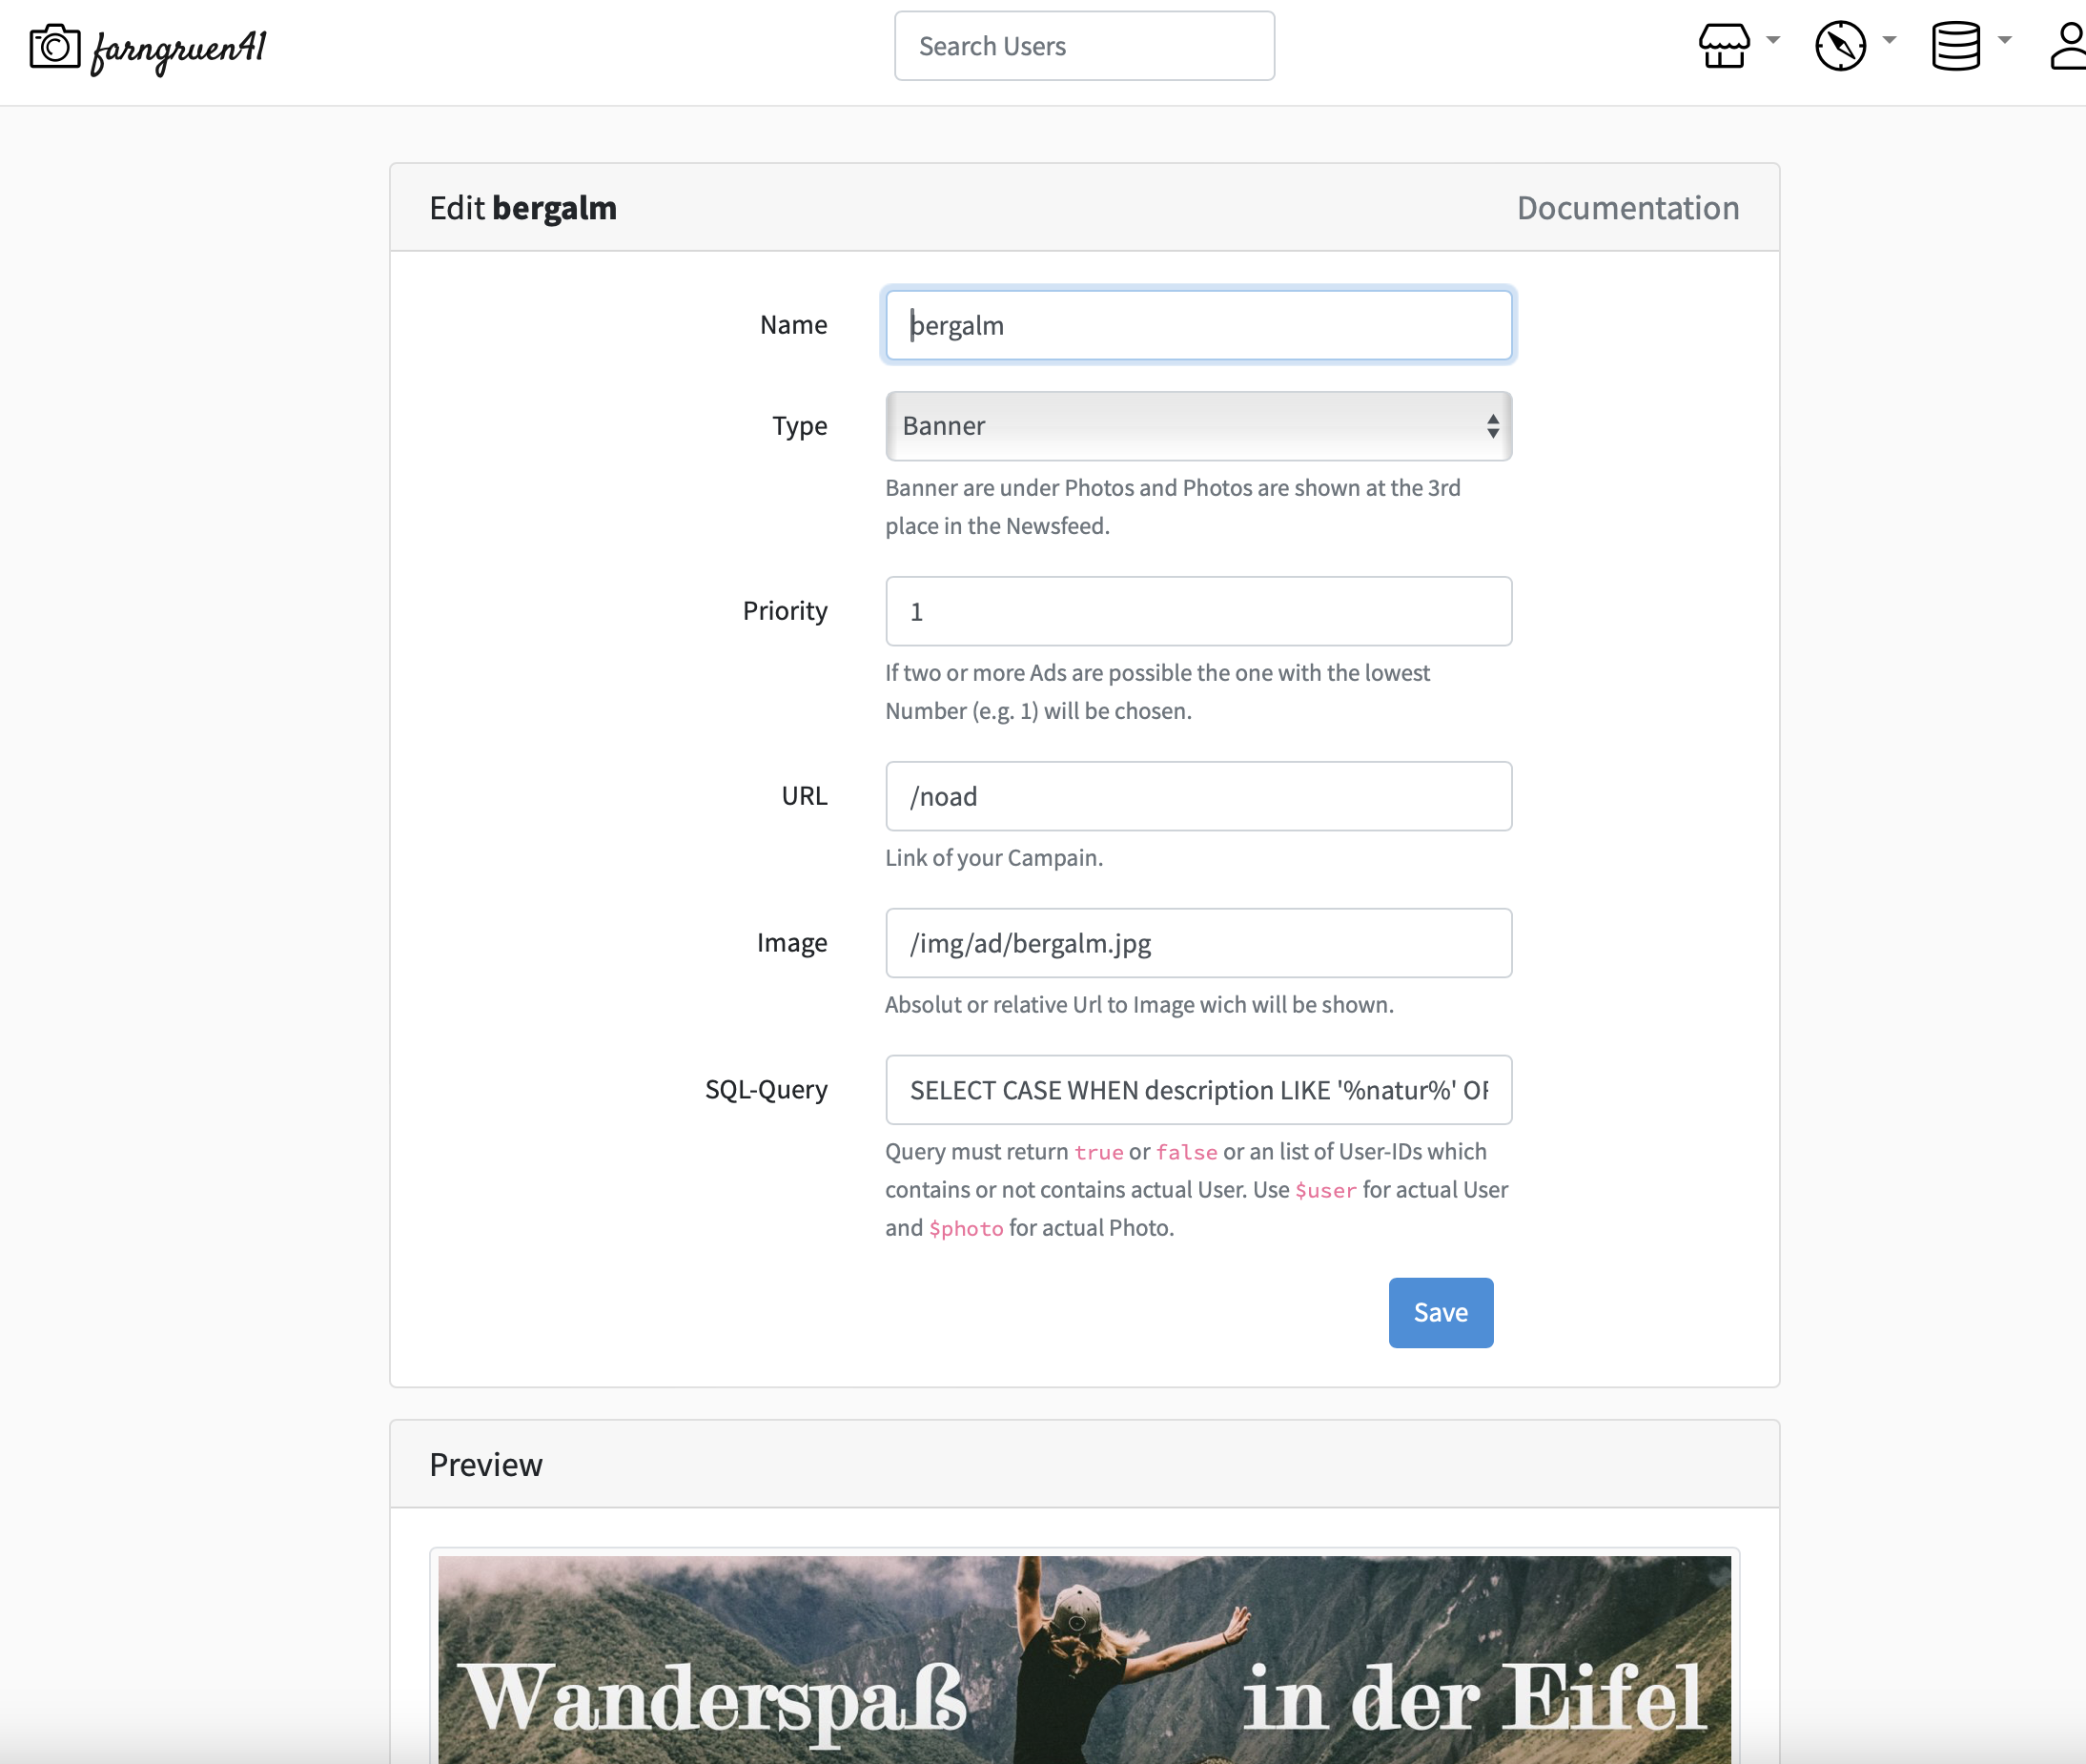
\includegraphics[width=0.7\linewidth]{GrundlagenInfo/06_Daten/Figures/screenshot-ads2}
  \caption{Beispielkampagne}
  \label{fig:screenshot-ads2}
\end{figure}

Als erstes sehen wir den (frei wählbaren) Kampagnen-Namen \texttt{bergalm}. Wir sehen auch dass die Werbung vom Typ ``banner'' ist, sie wird also bei Fotos angezeigt. Nebst weiteren Informationen sehen wir insbesondere zuunterst die ``SQL-Query'', also die SQL-Abfrage, mit der eine Werbung personalisiert wird.
Für diese Natur-Werbung haben wir folgende Abfrage:

\begin{lstlisting}
SELECT CASE 
	WHEN description LIKE '%natur%' 
	OR   description LIKE '%landschaft%' 
	OR   description LIKE '%berg%' THEN true 
	ELSE false 
END 
FROM photos 
WHERE id=$photo
\end{lstlisting}

Diese Abfrage wird nun auf der Webseite für jedes Foto ausgeführt, um zu sehen, ob die Werbung zum Foto passt.

Wir sehen zuerst, dass die Kolonne \texttt{description} der Tabelle \texttt{photos}, also die Kolonne, die Hashtags speichert, auf Texte wie ``Natur'', ``Landschaft'' und ``Berg'' abgesucht wird. Falls so ein Text vorhanden ist in den Hashtags des Fotos, wird der Wert \texttt{true} zurückgegeben, und somit wird die Werbung potentiell angezeigt, andernfalls wird der Wert \texttt{false} zurückgegeben. Auf der letzten Zeile sehen wir eine Variable \lstinline|$photo|, mit welcher jedes Foto der gesamten Webseite nach den genannten Kriterien abgesucht werden kann.

\begin{myexercise}
  Verändern Sie den SQL-Befehl so, dass die Werbung auch für Fotos mit dem Hashtag ``\texttt{\#Wasser}'' angezeigt werden. Testen Sie danach, ob es geklappt hat, indem Sie Fotos mit diesem Hashtag suchen. Sie können auf folgender URL überprüfen, ob es geklappt hat: \url{[ihrefarbe].instahub.org/p/1517}.
  \begin{myanswer}
    \begin{lstlisting}
SELECT CASE 
	WHEN description LIKE '%natur%' 
	OR   description LIKE '%landschaft%' 
	OR   description LIKE '%wasser%' 
	OR   description LIKE '%berg%' THEN true 
	ELSE false 
END 
FROM photos 
WHERE id=$photo
\end{lstlisting}
  \end{myanswer}
\end{myexercise}

\begin{mychallenge}
  Erstellen Sie eine neue Werbekampagne (s. \cref{fig:screenshot-ads1}).
\end{mychallenge}

\begin{mychallenge}
  \begin{table}[H]
    \centering
    \begin{tabular}{r|l}
      \emoji{chequered-flag}            & Gemeinsam ein soziales Netzwerk verwalten \\\hline
      \emoji{family-man-woman-girl-boy} & 3er- bis 4er-Gruppen                      \\\hline
      \emoji{stopwatch}                 & ca. 25 min.
    \end{tabular}
  \end{table}

  Um sich ein Konto auf einer Seite einer anderen Person zu erstellen:
  \begin{itemize}
    \item Bestimmen Sie jemanden als \textcolor{RoyalBlue}{AdministratorIn} und verwenden Sie nur die Webseite dieser Person, also z.B. \url{https://purpurrot21.instahub.org}. Die anderen Personen sind  \textcolor{ForestGreen}{BenutzerInnen}.
    \item \textcolor{ForestGreen}{BenutzerInnen}: Gehen Sie auf die von der Administratorin erstellte Webseite (\url{https://namedesnetzwerks.instahub.org}, wobei ``\texttt{namedesnetzwerks}'' ersetzt werden muss) und erstellen Sie ein neues Konto für sich.
    \item \textcolor{RoyalBlue}{AdministratorIn}: Die neuen Accounts der \textcolor{ForestGreen}{BenutzerInnen} muss dann von Ihnen als \textcolor{RoyalBlue}{AdministratorIn} aktiviert werden, indem Sie den User suchen, auf ``Bearbeiten'' und dann ganz unten auf ``Account ist freigeschaltet'' klicken.
    \item \textcolor{RoyalBlue}{AdministratorIn} und \textcolor{ForestGreen}{BenutzerIn}: Posten Sie nun falls Sie möchten Bilder in den sozialen Netzwerken Ihrer Kollegen, vergeben Sie Likes, folgen Sie anderen und kommentieren Sie fleissig in den anderen Netzwerken (max. 5 Minuten).
    \item Erstellen Sie nun personalisierte Werbungen für Ihre KlassenkameradInnen (s. \cref{fig:screenshot-ads1}).
  \end{itemize}
\end{mychallenge}
